
\chapter{Bisherige Arbeiten}

%-------------
\section{Ziva}

\begin{itemize}
 \item Ziva VFX Maya Plugin zur Erstellung von Charakteren und Simulation von biomechanischen Bewegungen \url{https://zivadynamics.com/}
 \item Charaktererstellung in Ziva beginnt mit der Modellierung des Skeletts. Knochen mit Animationen werden als Alembic-Datei gespeichert und dann in "`Ziva-Knochen"' konvertiert. \url{https://discover.therookies.co/2019/06/01/vfx-in-9-steps/}
\end{itemize}

%---------------------------
\section{ZSpheres in Zbrush}

\begin{itemize}
 \item \url{http://docs.pixologic.com/user-guide/3d-modeling/modeling-basics/creating-meshes/zspheres/},\\ Beispielvideo: \url{https://www.youtube.com/watch?v=Wl0XK6ggUOA}
 \item Möglichkeit ein "`Skelett"' aus Kugeln zu erstellen. Definiert aber eher die grobe Außenhaut mit Zusatzinformationen dazu wo die Gelenke sind.
\end{itemize}

%----------------------
\section{3DS MAX Biped}

\begin{itemize}
 \item \url{https://knowledge.autodesk.com/support/3ds-max/learn-explore/caas/CloudHelp/cloudhelp/2019/ENU/3DSMax-Character-Animation/files/GUID-2F6BC5D1-DD45-4C2E-AC3A-D8C6E0F5DEB1-htm.html}
 \item Möglichkeit Skelett in einen fertig modellierten Körper einzupassen. 
 \item Skelette sind schon vorgefertigt.
 \item v.a. für menschliche Skelette, aber auch (limitiert) anpassbar auf Tiere
\end{itemize}

%---------------------------------
\section{Forensik und Archäologie}

\begin{itemize}
 \item forensische Gesichstrekonstruktion ist spezialisiert auf Menschen und verwendet Zusatzinformationen wie Stockfotos von Gesichtsmerkmalen (\url{https://en.wikipedia.org/wiki/Forensic_facial_reconstruction})
 \item Rekonstruktion von Tieren in der Archäologie anhand des Skeletts v.a. durch Künstler (?)
\end{itemize}


%----------------------
\section{No Man's Sky}

\begin{itemize}
 \item Webseite \cite{NoMansSky}
 \item "`For creatures, basic templates of creatures that exist on the Earth were created and then manipulated by the system, changing everything from height, weight, bone density, voice pitch, what it eats, and its behaviors, even creating variation within the species."' (\url{https://nomanssky.fandom.com/wiki/Biology})
 \item "`Creatures were often generated by mixing and matching random parts from a library, and then adjusting the underlying skeleton so that the creature appeared realistic; a creature with a tiny body could not support a giant head, for example."' (\url{https://en.wikipedia.org/wiki/Development_of_No_Man\%27s_Sky})
 \item Zunächst Generierung von äußerem 3D-Modell, dann Anpassung der Knochen.
\end{itemize}

%-----------------
%-----------------
\chapter{Biologie}

\begin{itemize}
 \item "`Wirbeltiere (Vertebrata) [\dots] Von vielen Zoologen wird heute der Begriff Schädeltiere (Craniota) für dieses Taxon bevorzugt. Diese Auffassung berücksichtigt, dass die Rundmäuler, wie auch einige andere Wirbeltiere, als Achsenskelett keine Wirbelsäule, sondern eine Chorda dorsalis haben. Doch allen Wirbeltieren gemein ist ein verknöcherter oder knorpeliger Schädel; sein Vorhandensein gehört somit zu den gemeinsam abgeleiteten Merkmalen (Synapomorphien) dieser Chordaten-Gruppe."' (\url{https://de.wikipedia.org/wiki/Wirbeltiere}) $\rightarrow$ Beschränkung auf Schädeltiere mit Wirbelsäule
 \item "`Dem Skelett der Wirbeltiere sind viele Gemeinsamkeiten ansehbar, trotzdem unterscheidet es sich, je nach Lebensraum und Anforderungen, teilweise erheblich. Mit diesen Gemeinsamkeiten und Unterschieden beschäftigt sich die Vergleichende Anatomie."' (\url{https://de.wikipedia.org/wiki/Skelett#Wirbeltiere}) Notizen zu \cite{Vergleichende_Anatomie} siehe Anhang \ref{appendix_vergleichende_anatomie}.
 \item Das Skelett eines Wirbeltiers ist nicht unbedingt zusammenhängend.
 
 \item "`Säugetiere haben in der Regel sieben Halswirbel."' Es kann aber zwischen $6$ und $31$ variieren. Vögel haben zwischen $10$ und $31$ und zwei Tiere haben $6$ Wirbel. (\url{https://de.wikipedia.org/wiki/Halswirbel})
 
 \item Form der Wirbelsäule siehe \url{https://de.wikipedia.org/wiki/Wirbels\%C3\%A4ule}
\end{itemize}

%-------------
%-------------
\chapter{Idee}

\begin{enumerate}
 \item Erzeugung eines Wirbeltierskeletts
 \item Erzeugung von Muskeln (future work)
 \item Erzeugung von Haut (future work / kurz ausprobieren)
 \item Erzeugung von vielen Skelettvarianten bei Eingabe eines Skeletts (nur wenn es relativ leicht möglich ist)
\end{enumerate}

%---------------
\section{Skelett}

\begin{itemize}
 \item Iterative Erzeugung eines Skeletts durch eine probabilistische kontextfreie (?) Grammatik, die so erweitert ist, dass sie nicht ein einfaches Wort erzeugt, sondern einen Baum von Zeichen (nötig für Extremitäten). Verwendung von paramterischen L-Systemen \cite{Paramteric_L-Systems} könnte sinnvoll sein.
 \item Regeln sind nicht wirklich eine Grammatik, da fast jedes nichtterminale Literal nur einmal vorkommt, wenn es für jedes Körperteil andere Regeln gibt. Oder ist es möglich so zu abstrahieren, dass z.B. Arme und Beine den gleichen/ähnlichen Regeln unterliegen? Ist das sinnvoll? \todo{Abstraktionsgrad, Art der Regeln}\\%TODO
 Außerdem ist das Skelett nicht unbedingt zusammenhängend (siehe Biologie). $\rightarrow$ Darauf achten, dass das nicht von Algorithmus verlangt wird
 \item Regeln wichtig, die dafür sorgen, dass das Tier am Ende auch funktional ist.
 \item Darstellung des Skeletts in "`sinnvoller"' Pose.
 \item Beachte, dass Tier nicht umfällt: berechne Drehmomente um Kontaktpunkte mit Boden. Dafür sind aber Muskeln bzw.\ Masse wichtig $\rightarrow$ Schätzung der Masse anhand der Knochengröße bzw.\ Größe der Bounding Box?
 \item Der Zufall ist eingeschränkt durch Eingabeparameter oder Benutzereingabe (siehe Interaktivität). Ähnliche Parameter sollten zu ähnlichem Tier führen. Parameter könnten folgendes beschreiben:
 \begin{itemize}
  \item äußere Einflüsse (Klima, Terrain, Lebensraum,\dots)
  \item Proportionen (länge der Extremitäten, Kopfgröße,\dots)
  \item Anzahl vorhandener Gliedmaßen / Zehen / \dots
 \end{itemize}

 \item Ein Skelett besteht aus Knochen, Gelenken und deren (relativen) Positionen und Orientierungen.
 \item Ein Knochen ist im einfachsten Fall ein Zylinder (Strecke) mit Länge und Radius, kann aber auch eine konvexe Kurve mit einem Radius sein.
 \item Ein Gelenk hat keine Ausdehnung (?). Es ist das Verbindungsstück zwischen zwei oder mehr Knochen und legt fest wie die Knochen sich relativ zueinander bewegen können. Werden mehr als zwei Knochen verbunden ist es einfach eine feste Verbindung.
 \item Skelett darf nicht zu abstrakt sein, da es sonst zu wenig Informationen zum konkreten Tier liefert.
 \item Ein detailliertes Skelett ist für Wesen sinnvoll, die es so noch nicht gibt bzw. wo man keine richtige Vorstellung davon hat wie es "`funktioniert"', z.B. bei mehr Gliedmaßen.
 \item Köpfe sind kompliziert $\rightarrow$ Auswahl an Köpfen bereitstellen (evtl. leicht skalier-/verformbar oder ineinander überführbar)
 \item Brustbein sorgt dafür, dass Skelett nicht mehr baumartig $\rightarrow$ erstmal weglassen, ist wahrscheinlich auch nicht unglaublich relevant
\end{itemize}

%- - - - - - - - - - - - 
\subsection{Extremitäten}

\begin{itemize}
 \item \url{https://de.wikipedia.org/wiki/Extremit\%C3\%A4tenevolution}
 \item "`Die paarigen Flossen von Fischen und Extremitäten von Tetrapoden sind insofern homologe Skelettelemente, als sie bei beiden an Schulter- und Beckengürtel ansetzen und die Extremitäten aus den paarigen Flossen evolutionär hervorgegangen sind.\cite{homology} Sie unterschieden sich jedoch im Knochenaufbau und in der Embryonalentwicklung, so dass ein evolutionärer Übergang aus den Einzelelementen schwer erklärbar ist."'\\
 $\rightarrow$ einfach ignorieren und trotzdem (erstmal) so modellieren?
\end{itemize}


%----------------
\section{Muskeln}

\begin{itemize}
 \item Die "`Hauptmuskeln"' verlaufen bei Wirbeltieren wahrscheinlich ähnlich, relativ zu den Knochen. Trotzdem unterscheiden sie sich recht stark.
 \item Knochen/Gelenke bekommen Zusatzattribute für Start- und Zielpunkte der Muskeln.
 \item Muskeln haben eine "`Dicke"' und aus Start- und Zielpunkt muss Kurve des Muskels generiert werden.
 \item Wie wird die genaue Form festgelegt? Muskeln irgendwie auf ihre "`Dicke"' aufblähen + Interaktion mit vorhandenen Elementen (andere Muskeln und Knochen) $\rightarrow$ future work
\end{itemize}

%-------------
\section{Haut}

\begin{itemize}
 \item Was für Algorithmen gibt es, die zu einem vorhandenen 3D-Modell eine Hülle mit gewissen Eigenschaften generieren? \\
 es gibt eine solche Funktion z.B. in AutoCAD \url{https://knowledge.autodesk.com/de/support/autocad/learn-explore/caas/CloudHelp/cloudhelp/2016/DEU/AutoCAD-Core/files/GUID-B7F99810-765E-4E7E-ABDD-275C64147CCC-htm.html}
 \item Einfach nur eine Hülle mit gewissem Abstand sieht wahrscheinlich sehr unrealistisch aus. "`Bony Landmarks"' (Stellen an denen das Gewebe über den Knochen sehr dünn ist) könnten helfen (siehe \url{https://www.proko.com/landmarks-of-the-human-body/}) oder "`bone weights"'
\end{itemize}

%-----------------------
\section{Interaktivität}

\begin{itemize}
 \item Eine Anwendung, bei der nach Eingabe von Parametern sofort das komplette Tier generiert wird, ist weniger hilfreich als eine, bei der schrittweise Teile davon generiert werden können (und auch rückgängig gemacht werden können)
 \item Teile, die einem nicht gefallen, sollten geändert werden können
 \item Änderungen können Auswirkungen auf den Rest des Körpers haben (durch Regeln) bzw. manche Änderungen sind nicht möglich
 \item Könnte verwendet werden um schnell verschiedene Möglichkeiten zu testen
\end{itemize}

%------------
\section{PCA}

 \emph{Primary Component Analysis} (PCA) wird mit dem Ziel angewendet herauszufinden was die "`Hauptdimensionen"' sind, in denen sich Skelette unterscheiden.
 
 Die Eingabe für eine PCA ist eine Menge von Punkten. Diese Punkte repräsentieren einzelne Instanzen dessen, was untersucht werden soll, hier ein Skelett. Für jede Eigenschaft des Skeletts hat der Punkt eine Dimension. Gegeben ist also eine Menge von Punkten $P$ mit jeweils $d$ Dimensionen. Sie bilden im $d$-dimensionalen Raum einen Ellipsoid.
 
 Das Ziel der PCA ist herauszufinden wo die Achsen des Ellipsoids liegen, also wie die Eingabedimensionen miteinander korreliert sind. Interessant sind dabei die Achsen in deren Richtung die Daten die größe Streuung aufweisen.
 
 Um dies zu Berechnen wird zunächst der Mittelpunkt des Ellipsoids berechnet. Das ist der Punkt, der in jeder Dimension den Mittelwert aller Datenpunkte enthält. Dann wird der Mittelpunkt von den Eingabedaten abgezogen, also das Ellipsoid in den Ursprung des Koordinatensystems verschoben. Danach kann die Kovarianzmatrix aufgestellt werden, deren Einträge die Kovarianz zwischen den verschiedenen Achsen beschreibt.
 Die Eigenvektoren dieser Kovarianzmatrix sind dann die Achsen des Ellipsoids und die zugehörigen Eigenwerte geben an wie weit ausgedehnt das Ellipsoid in dieser Richtung ist.
 
 Will man nun herausfinden was die Haupteigenschaften eines Datenpunktes sind, stellt man ihn im neuen Koordinatensystem des Ellipsoids dar, also als gewichtete Summe der Eigenvektoren, und betrachtet dann nur die Dimensionen mit den größten Eigenwerten.

 %- - - - - - - - - - - - - - - - - 
 \subsection{Erhobene Daten für PCA}
 
 Flossen werden weder als Beine (egal ob mit oder ohne Bodenkontakt) noch als Flügel angesehen. \todo{sinnvoll?}
 
 \subsubsection{Skelettbilder}
 
 alle Bilder aus \cite{Spezielle_Zoologie} außer:
 \begin{itemize}
  \item Sinornis und Taube aus \cite{Vergleichende_Anatomie}
  \item Seekuh aus \cite{Zoologie25Wehner}
  \item Archaeopteryx, Eusthenopteron, Ichthyosaurus, Ichthyostega, Muraenosaurus, Urpferdchen aus \cite{Zoologie24Wehner}
  \item Pferd: \url{https://www.kosmos.de/content/buecher/ratgeber/pferde-reiten/vorwaerts-abwaerts-eine-frage-der-haltung/}
  \item Känguru \url{http://www.bildwoerterbuch.com/tierreich/beuteltiere/kaenguru/skelett-eines-kaengurus.php}
  \item Schwan \url{https://www.alamy.de/skelett-eines-schwans-osteographia-oder-die-anatomie-der-knochen-london-1733-quelle-47-ich-12-kapitel-v-saitenhalter-autor-cheselden-william-image226921369.html}
  \item Chamäleon \url{https://www.madcham.de/de/anatomie/}
  \item Gnu \url{https://lutzmoeller.net/Afrika/2007/Lutz-Juli/8-Gnu.php}
  \item Tyrannosaurus Rex \url{https://upload.wikimedia.org/wikipedia/commons/9/9f/Tyrannosaurus_skeleton.jpg}
  \item Dormedar \url{https://upload.wikimedia.org/wikipedia/commons/a/ac/Camel_Skeleton_-_Richard_Owen_-_On_the_Anatomy_of_Vertebrates_\%281866\%29.jpg}
  \item Strauß \url{https://www.scienceinschool.org/sites/default/files/articleContentImages/21/ostrich/issue21ostrich5_xl.jpg}
  \item Blauwal \url{https://www.quagga-illustrations.de/wp-content/uploads/2014/05/h0001705.jpg}
  \item Krokodil \url{https://de.depositphotos.com/210906852/stock-illustration-skeleton-crocodile-vintage-line-drawing.html}
  \item Giraffe \url{https://de.wikipedia.org/wiki/Giraffen#/media/Datei:Giraffe_skeleton.jpg}
 \end{itemize}

 
 \subsubsection{Gewicht}
 \begin{itemize}
  \item Gewicht: Durchschnittsgewicht eines ausgewachsenen Tieres in kg. Schwerstes Tier: Blaubwal, Maximum ist also 120 Tonnen \url{http://tierdoku.com/index.php?title=Blauwal}
  \item Durschnittsgewicht (Warmblut-)Pferd: 600 kg \url{https://www.reitarena.com/de/blog/blog-post/2015/03/03/das-pferd-grundlegende-fakten.html}
  \item Afrikanischer Elefant 4000kg: \url{https://de.upali.ch/gewicht-und-grosse/}
  \item Amerikanischer Flussbarsch 2kg: \url{http://tierdoku.com/index.php?title=Amerikanischer_Flussbarsch}
  \item Archaeopteryx wird zu Vögeln gerechnet, Gewicht 1kg \url{https://de.wikipedia.org/wiki/Archaeopteryx}
  \item Brachiosaurus (Reptil \url{http://www.biologie-schule.de/brachiosaurus-steckbrief.php}), 23 - 44 Tonnen \url{https://de.wikipedia.org/wiki/Brachiosaurus}
  \item Dimetrodon Reptil, 250kg \url{https://de.wikipedia.org/wiki/Dimetrodon}
  \item Elster 0,2kg \url{https://de.wikipedia.org/wiki/Elster}
  \item Forelle 10-50kg (je nach Art) \url{https://de.wikipedia.org/wiki/Forelle}
  \item Fregattvogel (Bild nicht verwendet, da nicht im Stand, sondern im Flug abgebildet) 0,6 - 1,6kg \url{https://de.wikipedia.org/wiki/Fregattv\%C3\%B6gel}
  \item Grönlandwal 50-100 Tonnen \url{https://de.wikipedia.org/wiki/Gr\%C3\%B6nlandwal}
  \item Ichthyornis 0.3kg \url{http://dinodata.de/animals/birds/pages_i/ichthyornis.php}
  \item Ichthyosaurus Fisch ca 90kg \url{https://www.tiere-online.de/sonstige-tiere/dinosaurier/ichthyosaurus/}
  \item Ichthyostega 80kg \url{https://dinosaurierwelt.com/ichthyostega/}
  \item Kaffernbüffel 350 - 900kg \url{https://de.wikipedia.org/wiki/Kaffernb\%C3\%BCffel}
  \item Kaninchen je nach Art, grob 1kg
  \item Klippschliefer 2-5kg \url{https://de.wikipedia.org/wiki/Klippschliefer}
  \item Koboldmaki 0,1kg \url{https://de.wikipedia.org/wiki/Koboldmakis}
  \item Landschildkröte unterschiedlich grob 50kg
  \item Ohrenrobbe 25-500kg \url{https://de.wikipedia.org/wiki/Ohrenrobben}
  \item Panzerspitzmaus 100g \url{https://de.wikipedia.org/wiki/Panzerspitzmaus}
  \item Parasaurolophus walkeri 4-5 Tonnen \url{http://tierdoku.com/index.php?title=Parasaurolophus_walkeri}
  \item Peloneustes philarchus 100kg \url{https://de.wikipedia.org/wiki/Peloneustes}
  \item Pottwal bis 50 Tonnen \url{https://de.wikipedia.org/wiki/Pottwal}
  \item Rothirsch 80-350kg \url{https://de.wikipedia.org/wiki/Rothirsch}
  \item Seehund 100-150kg \url{https://de.wikipedia.org/wiki/Seehund}
  \item Sinornis 20g \url{http://dinodata.de/animals/birds/pages_s/sinornis.php}
  \item Stegosaurus 4,5 Tonnen \url{https://de.wikipedia.org/wiki/Stegosaurus}
  \item Taube unterschiedlich grob 1-2kg
  \item Thrinaxodon Reptil "`ein paar Pfund"' \url{https://www.thoughtco.com/thrinaxodon-1091887}
  \item Triceratops 6-12 Tonnen \url{https://de.wikipedia.org/wiki/Triceratops}
  \item Urpferdchen (Propalaeotherium) 30kg \url{https://de.wikipedia.org/wiki/Propalaeotherium}
  \item Schwan 14kg \url{https://de.wikipedia.org/wiki/Schw\%C3\%A4ne}
  \item Chamäleon 0,1 - 2kg \url{https://www.tierchenwelt.de/echsen/128-chamaeleon.html}
  \item Gämse 25-50kg \url{https://de.wikipedia.org/wiki/G\%C3\%A4mse}
  \item Gnu 140-250kg \url{https://de.wikipedia.org/wiki/Gnus}
  \item Schwein 100kg \url{https://de.wikipedia.org/wiki/Hausschwein}
  \item Känguru 2-90kg \url{https://de.wikipedia.org/wiki/K\%C3\%A4ngurus}
  \item Tyrannosaurus 9 Tonnen \url{https://de.wikipedia.org/wiki/Tyrannosaurus}
  \item Dromedar 300-700 kg \url{https://de.wikipedia.org/wiki/Dromedar}
  \item Afrikanischer Strauß bis 135kg \url{https://de.wikipedia.org/wiki/Afrikanischer_Strau\%C3\%9F}
  \item Frosch ca 10g \url{http://www.biologie-schule.de/frosch-steckbrief.php}
  \item Krokodil 100-1000kg \url{https://de.wikipedia.org/wiki/Krokodile}
  \item Schlange bis 100kg bei Riesenschlangen \url{https://de.wikipedia.org/wiki/Schlangen}
  \item Girafffe bis 2 Tonnen \url{https://www.tierchenwelt.de/huftiere/73-giraffe.html}
 \end{itemize}

 
 
%-----------------------------
%-----------------------------
\chapter{Technische Umsetzung}

\begin{itemize}
 \item Repräsentation des Zustands als Hierarchie von einzelnen Komponenten (terminale sowie nichtterminale).
 \item Übersetzung in ein 3D-Modell: zunächst .obj, später Verwendung von OpenGL mit vertex shadern etc.\
\end{itemize}


%---------------------------
\section{Programmiersprache}

\begin{itemize}
 \item Rust: nicht geeignet, da Datenstrukturen die zyklische Referenzen auf veränderbare Objekte verwenden nicht oder nur kompliziert umsetzbar sind.
 \item Java: scheint gut zu funktionieren. Es gibt Bibliotheken zum im-/exportieren von obj-Dateien und Unterstützung für OpenGL
\end{itemize}


%---------------------
\section{Dateiformate}

\begin{itemize}
 \item Einfachstes Format (nur für die Darstellung von 3D-Objekten ohne Zusatzinformationen): obj
 \item Erster Schritt: einfaches .obj erzeugen und mit Blender darstellen; einfach Knochen als Bounding Box darstellen
 \item Jeder Editor geht mit Muskeln und Gelenken anders um. Gibt es ein Dateiformat, das nicht speziell zu einem Editor gehört, dass Bedingungen an die Rotation von Gelenken speichern kann?
 \item Eigenes Format erzeugen? Dann bräuchte man Plugins um es in verschiedenen Editoren laden zu können. Viel verwendeter Editor: Houdini (kostenlos für Studenten aber nicht Open Source). Oder selbst darstellen (siehe Interaktivität).
\item Vorschlag von Jo: "`Memory dumps"', also direkt die structs aus dem speicher auf platte rausschreiben. Am besten wenn sie am Stueck liegen mit einem fwrite() und zurücklesen mit einem fread(). Es ist nuetzlich dazu am Anfang der Datei ein bisschen Metadaten zu speichern (magic number, version, array size etc).
\end{itemize}

%- - - - - - - - - -
\subsection{OpenSim}

\begin{itemize}
 \item \url{https://simtk-confluence.stanford.edu:8443/display/OpenSim/OpenSim+Documentation}
 \item Open Source Software Platform für die Modellierung uns Simulation von Menschen, Tieren, etc.\\
 aber vor allem gedacht zur Auswertung von experimentellen Daten
 \item Import von .obj Dateien möglich. Außerdem zusätzliche Daten wie Winkel von Gelenken über .mot oder .sto Dateien (eigenes Format von OpenSim, siehe \url{https://simtk-confluence.stanford.edu:8443/display/OpenSim/Preparing+Your+Data})
 \item Export in andere Dateiformate nicht möglich (?)
 \item für Download und Zugang zur "`Community"' Account nötig
 \item für Windows und Mac OS (Linux Support gibt es auch, ist aber schwieriger: \url{https://simtk-confluence.stanford.edu:8443/display/OpenSim/Linux+Support})
\end{itemize}


%- - - - - - - -
\subsection{OBJ}

\begin{itemize}
 \item Beschreibung des Formats: \url{https://www.fileformat.info/format/wavefrontobj/egff.htm}
 \item Erzeugung mit Rust: obj\_exporter \url{https://docs.rs/obj-exporter/0.2.0/obj_exporter/index.html}
 \item Erzeugung mit Java: javagl Obj \url{https://github.com/javagl/Obj}, unterstützt auch Umwandlung von obj-Daten in Daten, die direkt für vertex buffer objects in OpenGL verwendet werden können
 \item Reicht wahrscheinlich für die ersten Dinge aus. Finetuning wird sowieso mit anderer Software gemacht
\end{itemize}

%- - - - - - - -
\subsection{FBX}

\begin{itemize}
 \item Verwendung am besten über Autodesk FBX SDK für C++. 
 \item Dokumentation: \url{http://help.autodesk.com/view/FBX/2019/ENU/} und \url{http://docs.autodesk.com/FBX/2014/ENU/FBX-SDK-Documentation/index.html}
 \item Es gibt auch fbxcel, eine FBX library für Rust. Ist aber relativ low level und nicht ganz offensichtlich wie zu verwenden.
 \item Einschränkungen für Gelenke können in FBX nicht gespeichert werden \url{http://docs.autodesk.com/FBX/2014/ENU/FBX-SDK-Documentation/index.html?url=cpp_ref/class_fbx_constraint.html,topicNumber=cpp_ref_class_fbx_constraint_htmlc57a3f99-513a-44a0-a24f-445e9077c99f}
\end{itemize}

%- - - - - - - - - -
\subsection{Alembic}

\begin{itemize}
 \item \url{www.alembic.io}
 \item Wird u.a. dafür verwendet Knochen (+ Animationen) in Ziva zu importieren
 \item Es kann mit Python (PyAlembic) und C++ verwendet werden.\\
 PyAlembic Doku: \url{http://docs.alembic.io/python/examples.html#pyalembic-intro}\\
 C++ API Refernce (enthält sehr wenig Infos): \url{http://docs.alembic.io/reference/index.html}
 \item Für Rust gibt es keine Bibliothek (?)
\end{itemize}

%-----------------------
\section{Interaktivität}

\begin{itemize}
 \item OpenGL
 \begin {itemize}
  \item SDL + OpenGL Tutorials \\ \url{http://headerphile.com/sdl2/opengl-part-1-sdl-opengl-awesome/}, \\ \url{http://www.sdltutorials.com/sdl-opengl-tutorial-basics}
  \item Daten direkt mit OpenGL erzeugen (laden als vertex und index array)
 \end {itemize}

 \item Benutzeroberfläche
 \begin{itemize}
  \item imgui (opengl/vulcan/3D view integriert) mit Rust oder C++: \url{https://github.com/ocornut/imgui}
  
  \begin{itemize}
   \item OpenGL und Imgui für Rust: \url{https://nercury.github.io/rust/opengl/tutorial/2018/02/08/opengl-in-rust-from-scratch-00-setup.html}, \url{https://github.com/michaelfairley/rust-imgui-sdl2}
   \item es gibt Java Bindings (\url{https://github.com/ice1000/jimgui}), aber Swing ist wahrscheinlich einfacher
   \item OpenGL scene $\rightarrow$ imgui: \url{https://gamedev.stackexchange.com/questions/140693/how-can-i-render-an-opengl-scene-into-an-imgui-window}
  \end{itemize}

  
  \item Java Swing Bibliothek und JOGL (Java OpenGL Binding) (\url{http://www.jogl.info})
 \end{itemize}
\end{itemize}

%------------------------
\section{Datenstrukturen}

%- - - - - - - - - - -
\subsection{Terminale}

\begin{itemize}
 \item Terminale zunächst als Bounding Box. Später werden sie durch Knochenmodelle ersetzt. Für jeden möglichen Knochen wird ein Modell gespeichert. Diese Modelle werden so skaliert, dass sie einen 1x1-Würfel ausfüllen. So kann dann später leicht die Skalierung auf diesen Würfel übertragen werden.
 
 \item Knochen: Bounding Box bzw. Skalierung in drei Raumrichtungen, Position, Orientierungen und Name bzw. ID (wird für Ersetzung benötigt).
 
 \item Knochen in Hierarchie anordnen und Position und Rotation relativ zu Elternelement angeben, da damit Erzeugung von Kindelementen einfacher $\rightarrow$ verwende homogene Koordinaten.\\
 Bei der Erzeugung von Elementen auf der Wirbelsäule ist das nicht einfacher. \todo{Hie\-rarchie nur von Elementen, die von der Wirbelsäule "`abzweigen"'? Oder ist gewisse Hierarchie in "`Endprodukt"' gewollt?} %TODO
 
 \item Gelenke: Position, Bewegungseinschränkungen für alle drei Richtungen. In einer Hierarchie verbindet das Gelenk ein Kindelement mit seinem Elternelement. Gelenk ist hier ein Punkt, der im Koordinatensystem des Elternelements angegeben wird, und um den das Koordinatensystem des Kindelements gedreht werden kann/soll.\\
 Das macht es sinnvoll ein Kindelement erst zu erzeugen, wenn das dazugehörige Elternelement terminal ist. Sonst weiß man noch nicht so genau wie das Gelenk aussehen soll. Mit etwas mehr Aufwand lässt sich das aber auch im Nachhinein noch anpassen\dots\\
 \todo{Bewegungseinschränkungen für bestimmtes Gelenk bei jedem Tier gleich? Wie Einschränkungen erzeugen?}, %TODO 
 
 \item Erzeugung von Kindelementen nicht nur von direktem Elternteil abhängig $\rightarrow$ Abhängigkeiten zwischen entfernten Teilen nötig; auch für Balance nützlich. "`Kommunikation"' über Überobjekt, das auch alle Einzelteile speichert. (SkeletonGenerator)
 \end{itemize}
 
%- - - - - - - - - - - -
\subsection{"`Wachstum"'}
 
\begin{itemize}

\item Lage der Wirbelsäule am Anfang festlegen, da sie der zentrale Teil des Körpers ist und die Lage der anderen Körperteile grob festlegt. Form variiert von Gerade (Fisch) bis geschwungener Hals und Schwanz (z.B. Giraffe). Mensch passt hier nicht ganz ins Schema $\rightarrow$ weglassen?
  
\item Position der Wirbelsäule wird zu Beginn durch ein, oder mehrere, Beziérkurve(n) festgelegt. Außerdem wird gestgelegt wo Elemente ansetzen, die nicht einfach Wirbel sind, \zb Extremitäten. Von diesen Punkten aus, kann das Skelett dann weiter "`wachsen"'. Diese Positionierung der Wirbelsäule legt die Länge und die Höhe des Tieres fest. Außerdem natürlich den Verlauf der Wirbelsäule, also \zb auch die Länge des Halses.\\
Regel, die zunächst sinnvoll klingt: Ansatzpunkte der Extremitäten an der Wirbelsäule können nur in Bereichen der Kurve sein, an denen die Steigung nahe null ist.

\item Wachstum unter Berücksichtigung verschiedener Randbedingungen wie Bodenposition, Anzahl Extremitäten etc.\ Bounding Box für Nichtterminale ist dafür aber nicht nötig.
  
\item Die Knochen sollen eine Hierarchie (Baum) bilden. Am besten ist ein Knochen in der Nähe es Schwerpunkts (oft wird die Hüfte verwendet). Die Hüfte gibt es aber nicht immer. Verwende ersten Wirbel nach dem Brustkorb (fals existent).
\end{itemize}

 
%- - - - - - - - - -
\subsection{Balance} 

Berechnung der Blance: Drehmomente der Knochen (benötigt Position der Knochen und Gewicht) $\rightarrow$ zunächst nicht nötig, da Position  der Wirbelsäule zu beginn mit Beziérkurve festgelegt wird

  \begin{itemize}
   \item Drehmoment $\vec{M} = \vec{r} \times \vec{F}$, mit Ortsvektor $\vec{r}$ vom Bezugspunkt des Drehmoments zum Angriffspunkt der Kraft $\vec{F}$. Betrag des Drehmoments $M = r \cdot F \cdot \textrm{sin}(\alpha)$, mit dem Winkel $\alpha$ zwischen $\vec{F}$ und $\vec{r}$.\\
   (\url{https://de.wikipedia.org/wiki/Drehmoment})
   
   \item Kraft, die auf Knochen wirkt: resultierende Kraft der Streckenlast, die durch zugewiesenes Gewicht erzeugt wird. Der Einfachheit halber einfach rechteckige Streckenlast annehmen, dann greift Kraft am Mittelpunkt der Strecke und $\vec{F} = \frac{1}{2} m g$\footnote{Die Formel zu rechteckigen Streckenlasten, die man so findet ist $\vec{F} = \frac{1}{2} L q_0$, mit Länge der Strecke $L$ und den auf der Strecke verteilten Einzellasten $q_0$, aber $L q_0 = m g$. Daraus folgt obige Formel.}, mit Masse $m$ und Erdbeschleunigung $g$\\ (\url{https://www.der-wirtschaftsingenieur.de/index.php/streckenlast/}, \url{https://www.youtube.com/watch?v=T1Sf8GPD4dc})
   
   \item Reduzierung des Problems auf zwei Dimensionen, da Körper so aufgebaut ist, dass er nur nach vorne oder hinten umkippen kann und nicht zur Seite.
   
   \item Damit Körper immer in Balance ist, muss auch nicht terminalen Teilen ein Drehmoment (und damit auch implizit ein Gewicht) zugewiesen werden. Werden aus diesen Nichtterminalen dann neue Teile generiert, so muss das Drehmoment bzw.\ die Summe der einzelnen Drehmomente gleich bleiben.
   
   \item Der Bezugspunkt für die Berechnung der Drehmomente ist der Schwerpunkt des Körpers, da sich dort alle durch das Eigengewicht wirkenden Drehmomente des Körpers zu null aufaddieren.\\ (\url{https://www.grund-wissen.de/physik/mechanik/drehmoment-und-gleichgewicht.html})\\
   Das heißt zu Beginn der Generierung muss der Schwerpunkt des Körpers festgelegt werden, damit die Drehmomente berechnet werden können. Das ist am Anfang aber sehr einfach, da das initiale Element die Bounding Box des Gesamten Skeletts ist. Also ist der Schwerpunkt der Mittelpunkt.
   
  \end{itemize}

%--------------------------------
%--------------------------------
\chapter{Implementierungsdetails}

%--------------------------------
\section{Transformationsmatrizen}

Jedes Element im Skelett speichert, relativ zu seinem Elternelement, die Position des Ursprungs seines Koordinatensystems. Um den Überblick über die Transformationsmatrizen bzw. Abbildungen behalten, die vom einen ins andere Koordinatensystem umwandeln, hier zwei Übersichtsgrafiken:

\begin{figure}
 \centering
 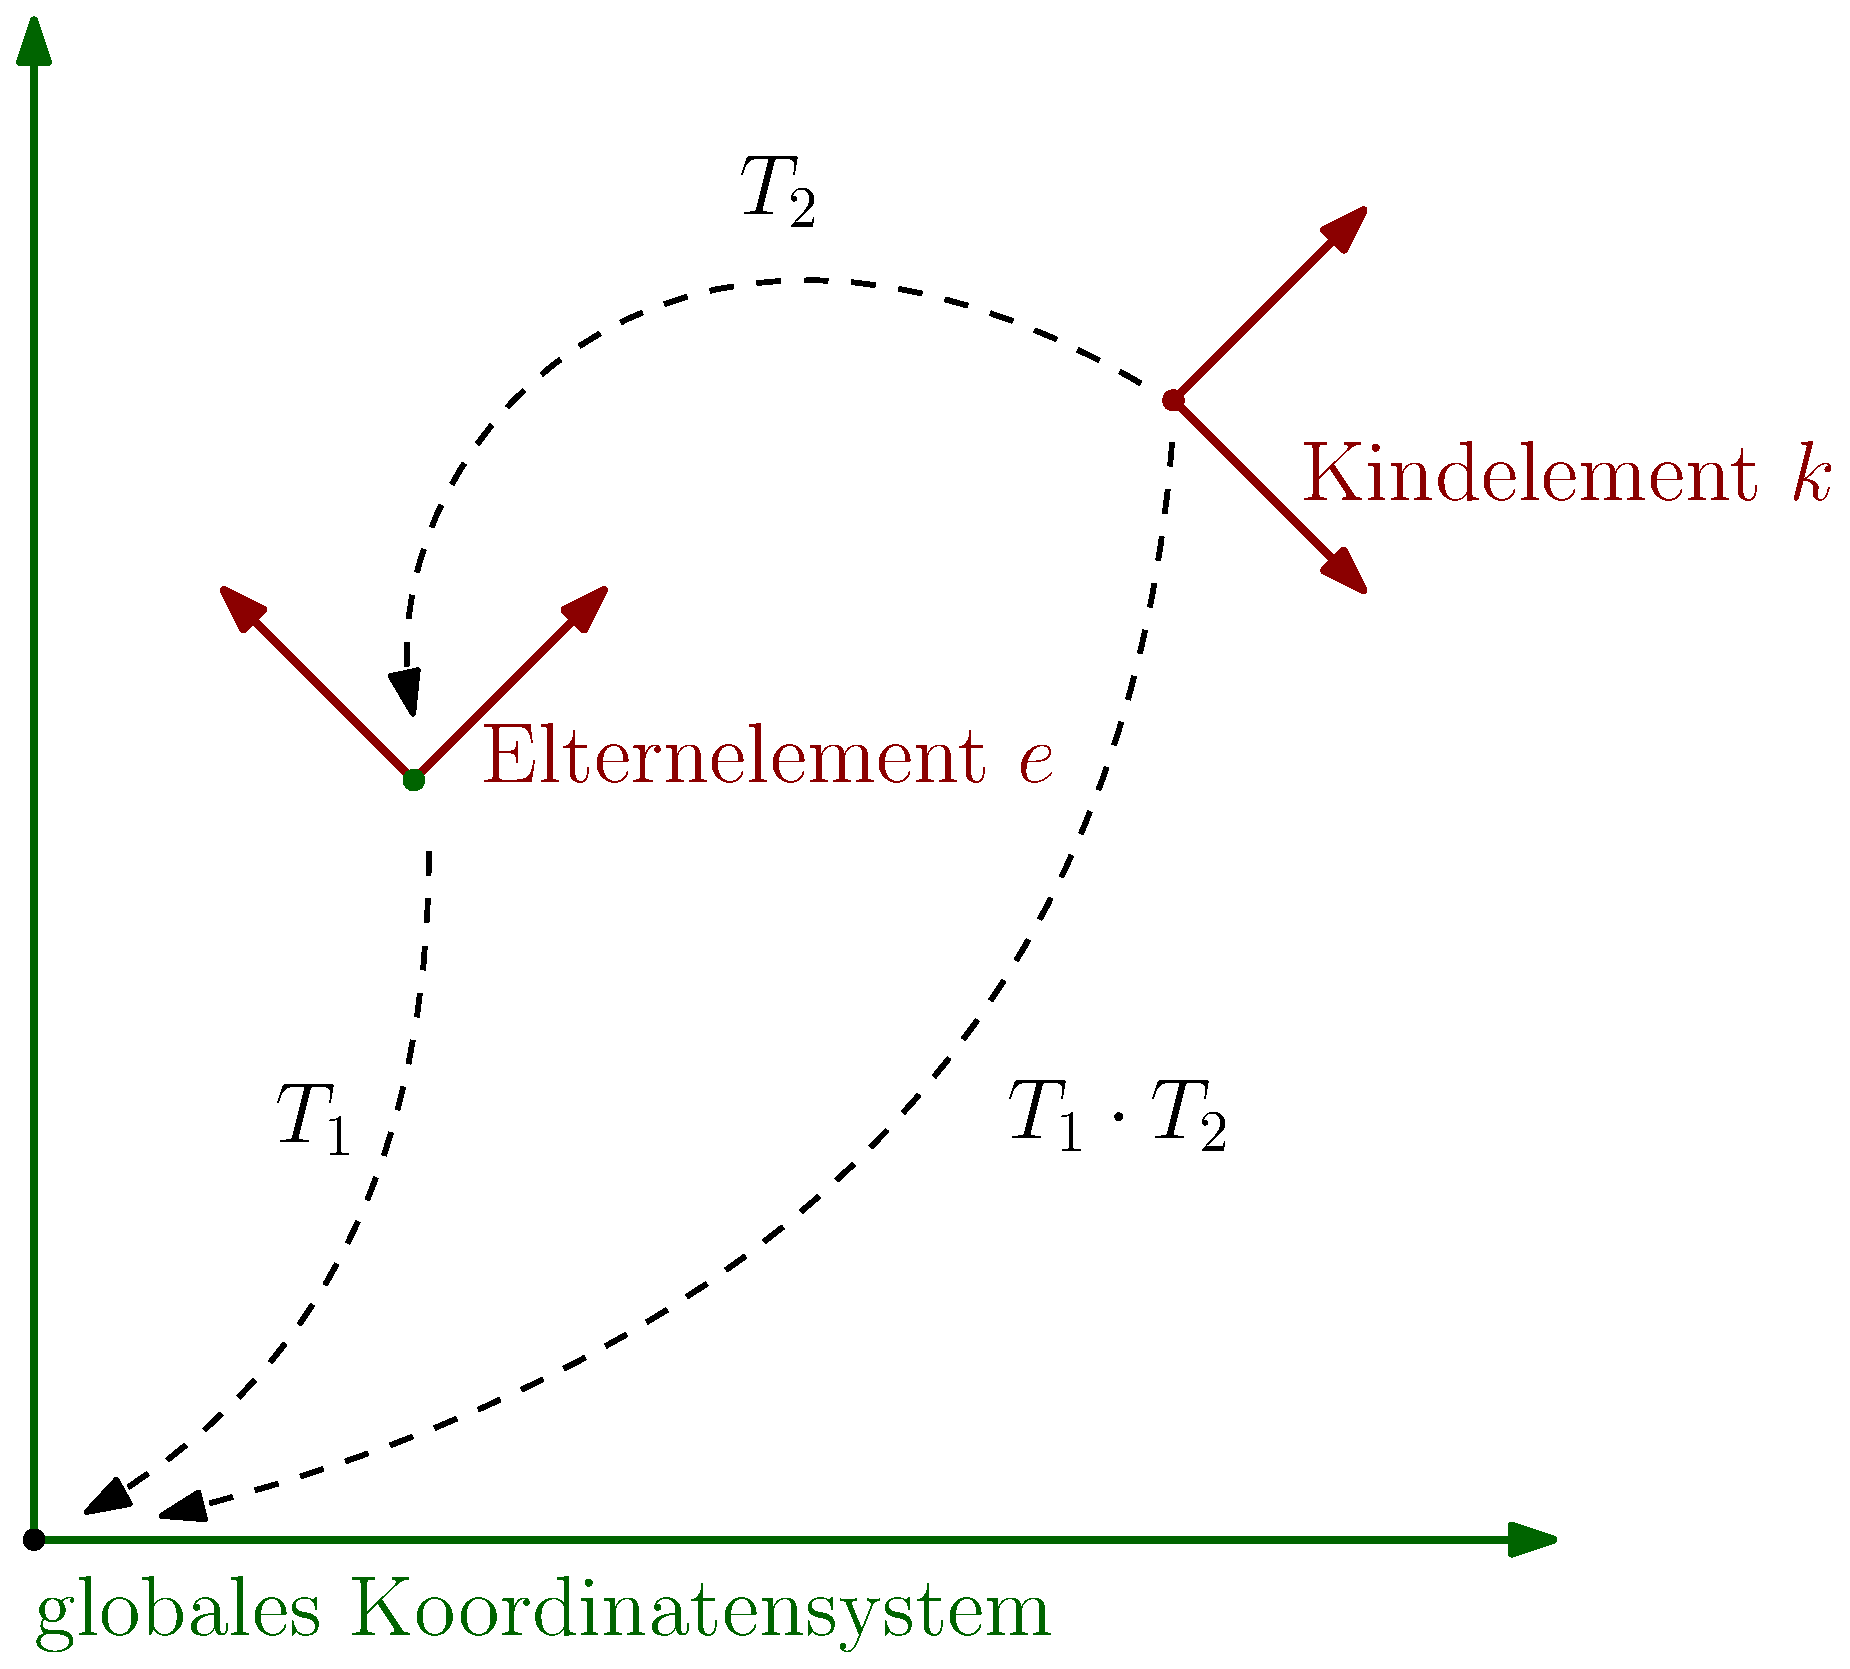
\includegraphics[width=0.6\textwidth]{graphics/transformation_matrices.eps}
 \caption{Gegeben sei das Element $e$. Die Abbildung, die die lokalen Koordinaten von $e$ in globale Koordinaten umrechnet sei $T_1$.
 Jedes Kindelement $k$ von $e$ speichert eine Transformationsmatrix $T_2$, die angibt wo der Ursprung des Koordinatensystems von $k$ relativ zum Koordinatensystem von $e$ liegt. Will mann nun Koordinaten von $k$ in globale Koordinaten umrechnen, benötigt man die Abbildung $T_1 \cdot T_2$.}
\end{figure}

\begin{figure}
 \centering
 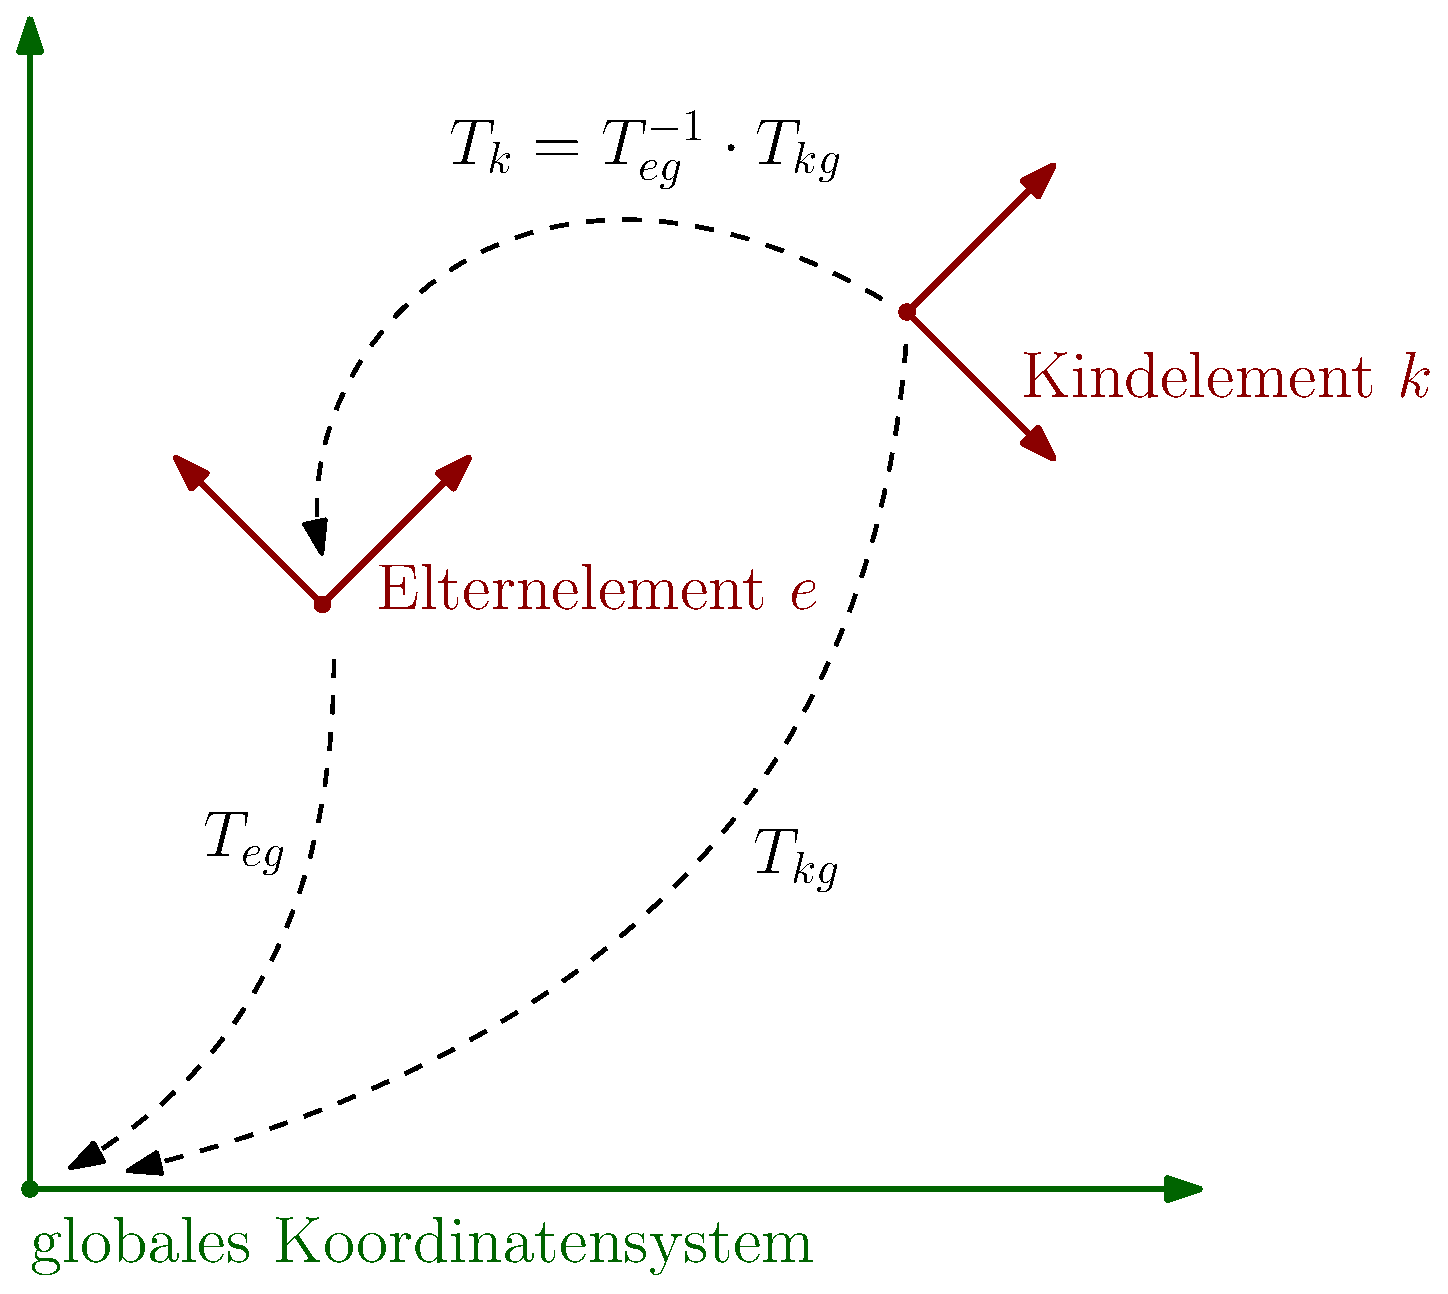
\includegraphics[width=0.6\textwidth]{graphics/transformation_matrices_spine.eps}
 \caption{Will man ein Element $k$ erzeugen, das Kindelement von $e$ ist und dessen globale Koordinaten bekannt sind, muss man die Abbildung berechnen, die die relative Position von $k$ angibt. Seien $T_1$ und $T_2$ jeweils die Transformationen in das globale Koordinatensystem von $e$ \bzw $k$. Dann ist die gesuchte Abbildung $T_1^{-1} \cdot T_2$.}
\end{figure}





